\section{XPS Measurements}
Three battery samples have been prepared for the \gls{xps} measurements for post mortem analysis. All the samples came from Sony US18650VTC3 round cells. The cells have a capacity of \SI{1.6}{\ampere\hour} and are operated in a voltage range from \SI{2.5}{\volt} to \SI{4.2}{\volt}. With a maximum discharge current of \SI{30}{\ampere} these cells can be categorized as high power cells, which is beneficial for any plating experiments at low temperatures since the cells have a comparably low internal resistance allowing for higher charge currents. Three cells have been prepared under different conditions. Two of the cells where only cycled once to bring them into the desired state, these are technically new cells. One of the cells was opened at 100\% \gls{soc} (furthermore referenced as sample A), the other cell was opened at 0\% \gls{soc} (sample B). The third cell was cycled for ten full cycles at \SI{-20}{\celsius} to produce lithium plating in the cell and then opened (sample C). All samples from the opened batteries have been taken from the outermost area of the jellyroll. The last analyzed sample was taken from pristine anode material that was not used inside a cell (sample D). This sample was used to get a reference of the graphite surface without any electrolyte or \gls{sei}. \par 

\begin{table}[h]
\centering
\begin{tabular}{clc}
\multicolumn{1}{l}{\textbf{Sample}} & \textbf{Description}    & \multicolumn{1}{l}{\textbf{Cycles}} \\
A                                   & Fully charged anode  & 1                                   \\
B                                   & Fully discharged anode     & 1                                   \\
C                                   & Plated anode            & 10                                  \\
D                                   & Prestine anode (no SEI) & -                                  
\end{tabular}
\caption{Anode samples for XPS measurements}
\label{xpsamples}
\end{table}

It has to be kept in mind that the pristine graphite is not from the same manufacturer as the anode samples from the opened batteries and is thus only used as a reference for the C1 peak and not further used in the interpretation of the results. All cells where opened inside a MBRAUN Unilab glove box under argon protective atmosphere with < \SI{10}{ppm} of moisture and oxygen concentration and then transferred to the XPS device inside a gas tight transport box. The XPS device has an attached mini glove box that was used to then transfer the samples from the transport box to the XPS test chamber. Within the mini glove box the samples have been exposed to a roughly \SI{100}{ppm} oxygen atmosphere for a few minutes before entering the high vacuum. It was unfortunately not possible to also measure the moisture content in the mini glove box during the transfer.  \par
For the \gls{xps} measurements a XPSDEVICEMISSING device was use with a base pressure of XXX Torr. The photo-electron source is a monochromatic \ce{Al} K$\alpha$ X-ray source ($h\nu$ = \SI{1486.7}{\electronvolt}).

\subsection{Preliminary Test: Influence of Sample Washing} 
Washing the samples taken from the battery with an appropriate solvent is often done prior to sensitive experiments. This is done to remove any battery electrolyte residue or electrolyte salt rests from the surface of the samples \cite{Yang.2010}. The solvents used for washing are often the same or similar to the solvents used in the electrolyte (e.g. \gls{dmc}). Mussa et al. however specifically mentions that washing can dissolve parts of the \gls{sei} and  does not recommend washing the samples after removing them from the battery. In this case washing can falsify the measurement results since the layer is not in the original sample state anymore. Somerville et al. \cite{Somerville.2016} did a study on the effects of washing on the surface film of graphite electrodes. They report that some authors could detect a higher sensitivity to atmosphere after the washing, which could be explained by the removal of a passivating surface film. The paper itself focused on the ratio of \gls{vc} in the electrolyte, an additive commonly used in \glspl{lib} to improve the formation of a stable \gls{sei}. They postulate that the washing removes the salt and the low boiling point solvents present in the surface layer (in this case \gls{ec}). Samples with different \gls{vc} ratios from 0 to 6 vol.\% have been prepared by them and analyzed using \gls{xps}, \gls{sem}, \gls{atr} and \gls{ftir}. They found two different films dependent in the \gls{vc} concentration with the two films showing a different \gls{sem} image as well as different behaviour in the material composition. The low \gls{vc} concentration film in contrary to the higher concentration film is also very sensitive to the washing process and for this film not only the salt deposits are removed but also \ce{LiF} and \ce{Li_xPF_y} which can only be found in the deeper layers of the \gls{sei}. Their results show clearly that whether washing it useful or not strongly depends on the composition of the electrolyte. \par
For the experiment in this work commercials cells have been used, so it is not possible to obtain any data about the composition of the electrolyte since battery producers generally do not make their internal electrolyte recipes public to the competition. For this reason it could not be determined beforehand whether washing the electrodes before testing is beneficial or harmful. So in the first test run measurements of one washed and one none-washed sample from each battery anode where analyzed and the results have been compared. The samples have been washed in two DMC baths for about 30 seconds each and then dried for one hour in the glovebox before they where mounted to the sample holder and transfered to the \gls{xps} device.

\begin{figure}[h]
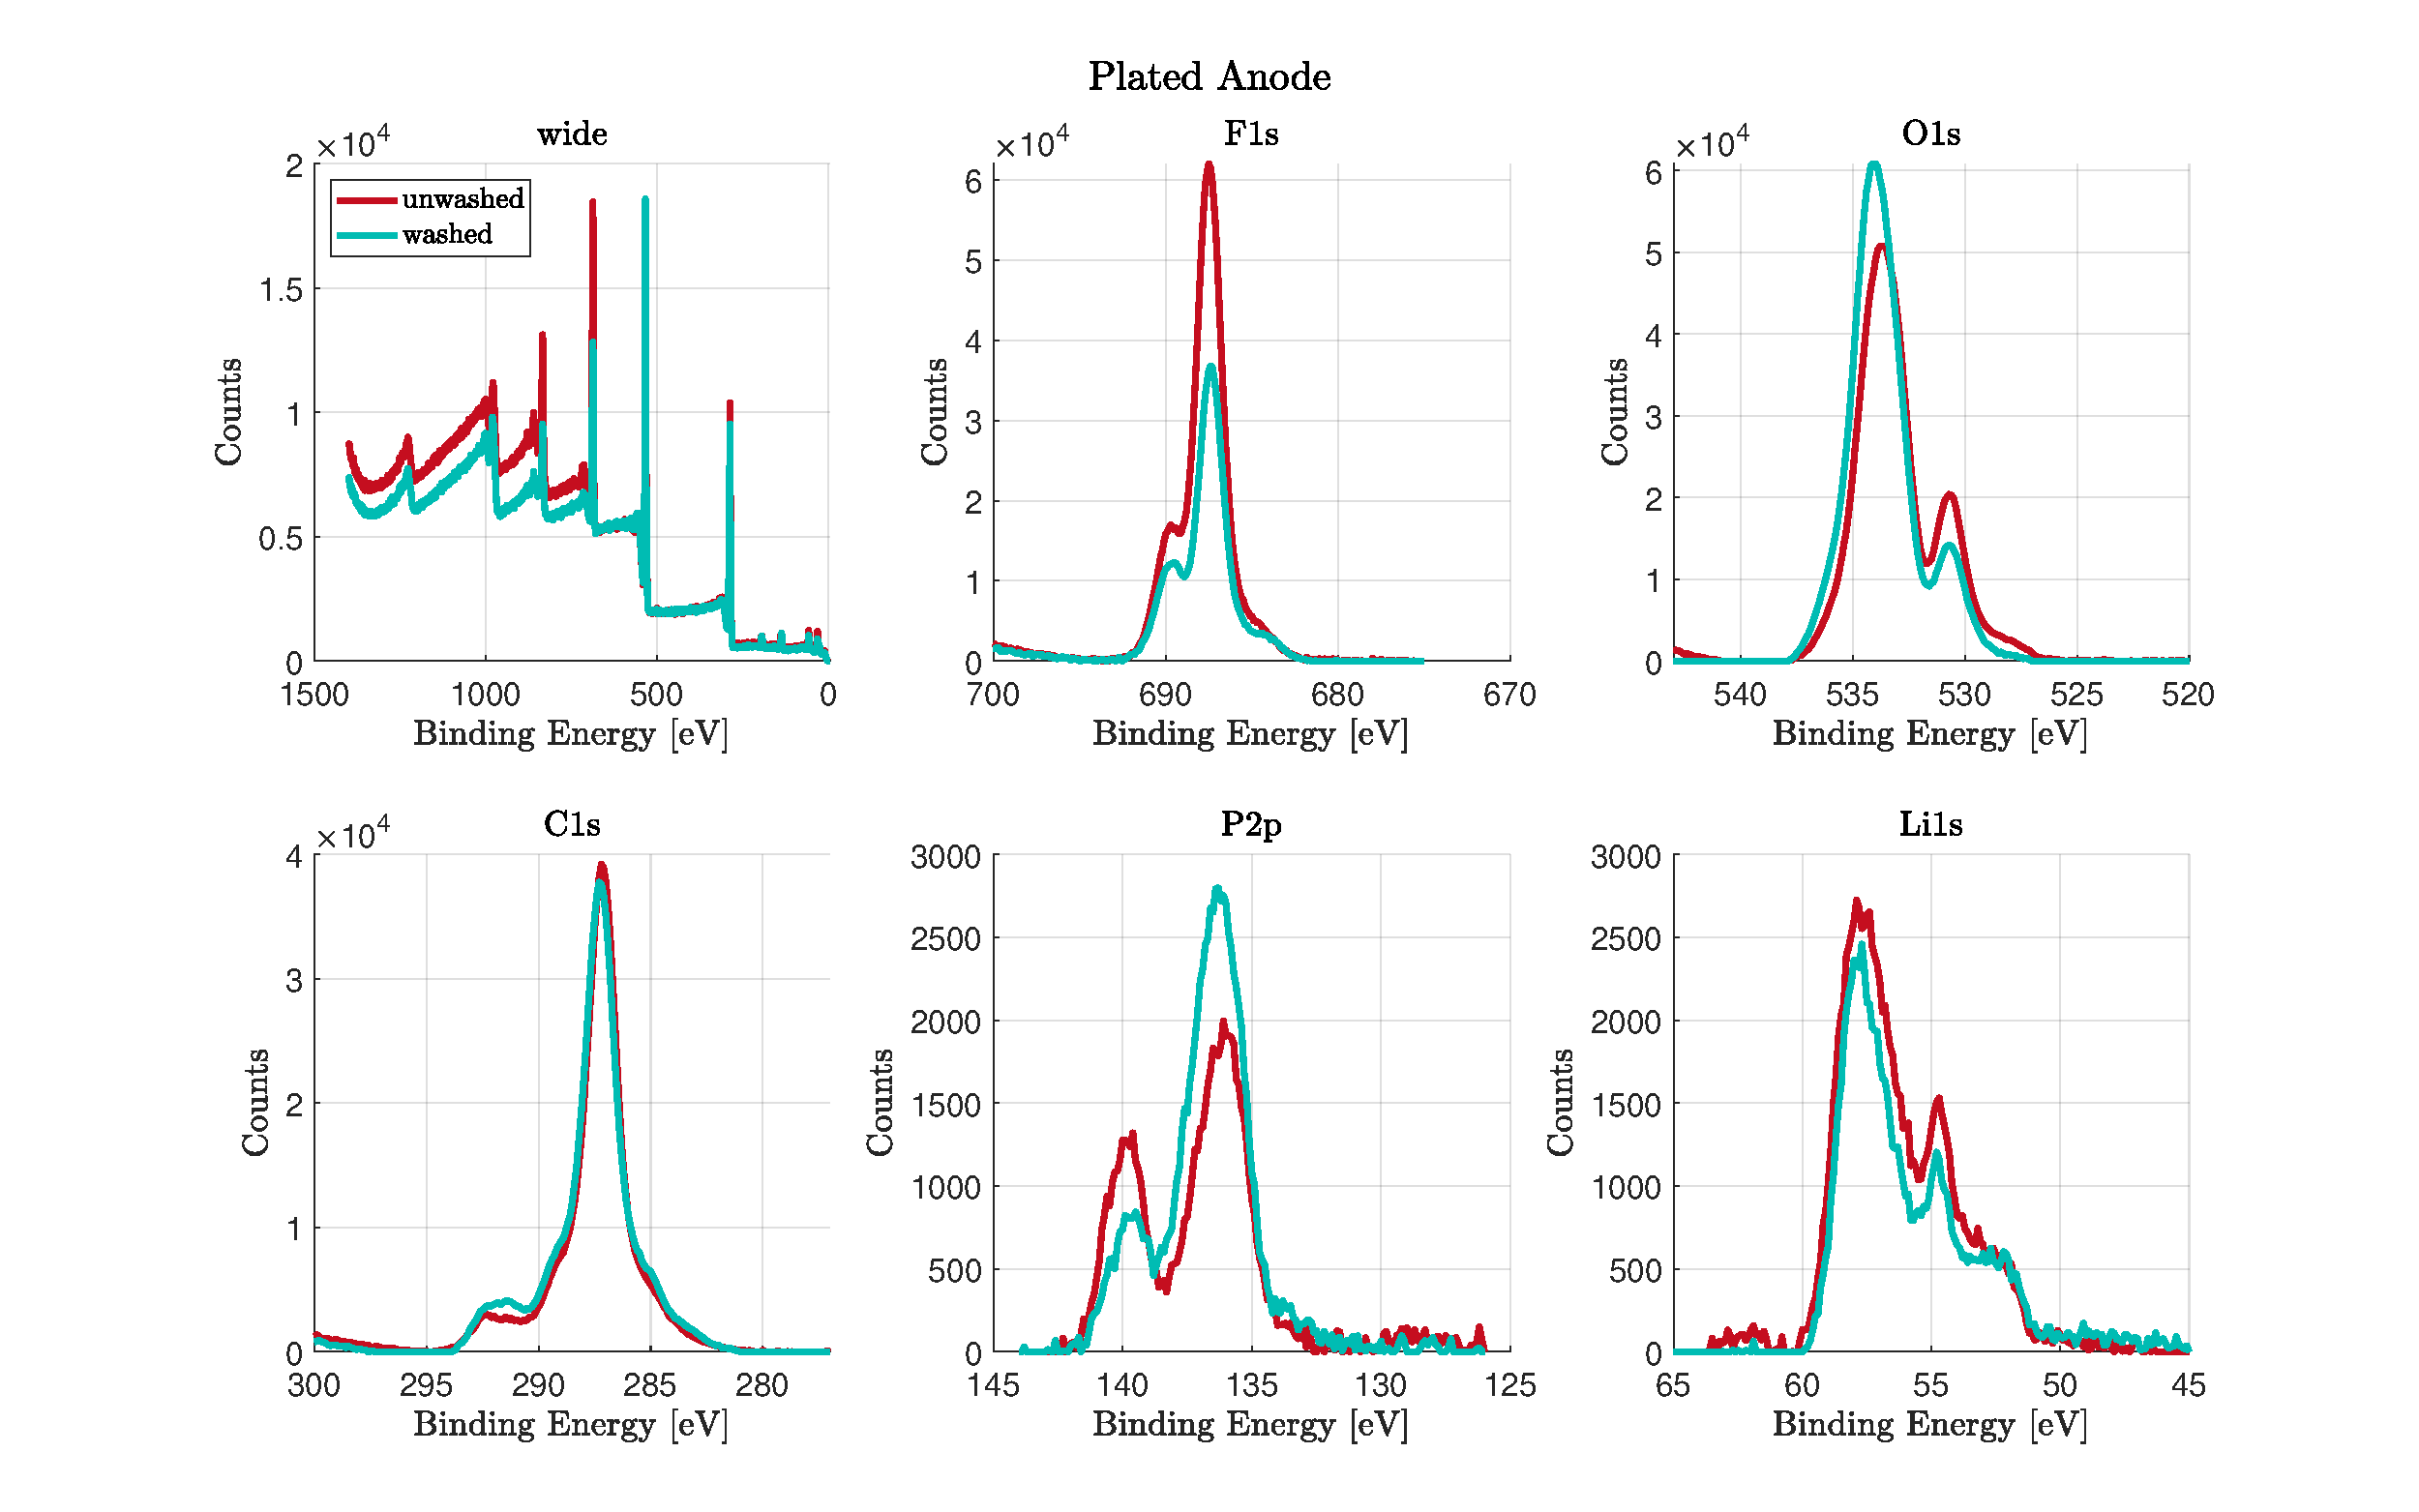
\includegraphics[width = \textwidth]{pictures/washed_unwashed_Plated Anode.pdf}
\caption[XPS spectra - 10 cycles of plating - washed vs unwashed]{XPS spectra of the anode after 10 cycles of plating (Sample C). Comparison between the washed and unwashed sample}
\label{wuplating}
\end{figure}